\documentclass{article}

\usepackage{amsmath}
\usepackage{graphicx}
\usepackage{amssymb}
\usepackage{placeins}

\title{EECS 325\\
       Project 2 Report}
\author{Devin Schwab (dts34)}
\date{December 7, 2012}

\begin{document}

\maketitle

\section*{Abstract}

This project investigated the correlation between Round Trip Times (RTTs), Hop count, and physical distance. Using a list of the top website of the world obtained from alexa.com, a tool was created that would find the total number of hops to reach a website and then measure the RTT. Using freegeoip.com an estimate of the physical distance was also calculated. The data shows that within the continent, under normal conditions that RTT is correlated with hop count, but distance is not strongly correlated with hop count, nor is distance strongly correlated with RTT.

\section*{Background}

Round Trip Time (RTT) is the time it takes for a piece of data to be sent to a destination and then returned. RTT often has an impact on the performance of a network application. Large RTT's can lead to slow performance and so in general it is desirable to have low RTT.  Intuitively it would seem that RTT would be correlated with both the physical distance, due to speed of light constraints, and with the number of routers (or hops) the data must pass through on its way to and back from the destination.

In order to determine the hop count from the computer running the tool to the list of destination sites the Time To Live (TTL) field of the IP header was utilized. When the TTL field of an IP header falls to zero the router which encountered the TTL will send back an Internet Control Message Protocol (ICMP) packet. ICMP is used for a number of things on the internet and each ICMP packet can be classified with a type and code. When the TTL expires a Type 11, code 0 ICMP packet is sent back to the original sender. Type 11 means ``Time Exceeded'' and Code 0 means ``Time to Live Exceeded in Transit''. Looking for Type 11, Code 0 ICMP packets allowed the tool created for this project to determine if the TTL was too low.

To determine if the TTL was too high the tool looked for Type 3, Code 3 ICMP packets. Type 3 means ``Destination Unreachable'' and Code 3 means ``Port Unreachable''. The reason these messages were expected was because the unlikely port of 33434 was used to collect the data. If the machine under investigation was actually running a service on this port then no ICMP message would be returned and the tool used for this project would not be capable of detecting machine or its RTT.

In order to match the ICMP packets the packet ID of the original packet sent was used. When an ICMP message is sent back it includes the packet headers of the original packet. Using the included packet headers in the ICMP message the original packet ID was checked for. If the packet ID's matched then this packet was utilized, if it didn't match then it was ignored.

This method of detecting if the machine was reached is flawed as server operators can configure their networks not to return ICMP messages. If no message was returned then an accurate measurement of RTT and Hop count could not be determined. 

Finally distance was calculated using the Haversine formula which calculates the distance between two latitude and longitude points. The Latitude and longitude points for each IP were determine via freegeoip.com which provides a URL which can be queried about any IP address. The response of the query is an XML formatted response which includes among other information Latitude and Longitude.

\section*{Procedure}

The tool used to collect the data from each website worked by sending out UDP packets to the unlikely port of 33434. If a Type 11, code 0 response came back then the tool knew that the TTL was too low. If a Type 3, Code 3 response came back then the tool knew that the TTL was either just right or too high. If no response was received the tool assumed that the TTL was too low and tried progressively higher TTL values, up to the maximum of 32. Any other response was treated like a timeout.

In order to cut back on the total number of packets sent a binary search algorithm was utilized. The TTL search space ranged from 1 to 32. Each iteration of the algorithm a packet with a TTL halfway between the lower and upper TTL bounds was sent. If the sent packet received a Type 3, Code 3 response then the upper TTL was lowered to the TTL value that was just sent. The RTT and TTL of that response were recorded. Any other response or a timeout and the lower TTL bound was raised to the value of the TTL just sent. When the upper and lower TTL bounds were adjacent to each other the algorithm was terminated. If a response had been received then it was recorded.

Initially the sites that were being tested were

\FloatBarrier
\begin{table}[h!]
  \begin{tabular}{|l|}
  \hline \\
  {\bf Website} \\ \hline
  yahoo.com \\ \hline
  alipay.com \\ \hline
  adultfriendfinder.com \\ \hline
  thefreedictionary.com \\ \hline
  bluehost.com \\ \hline
  nokia.com \\ \hline
  google.sk \\ \hline
  hidemyass.com \\ \hline
  nudevista.com \\ \hline
  nikkansports.com \\ \hline
  egotastic.com \\ \hline
  \end{tabular}
\end{table}
\FloatBarrier

However, only google responded to both by tool and to a UDP traceroute. Because its difficult to draw conclusions from a single data point other sites were chosen from the top 500 websites on alexa.com. Starting at page 1 of the top 500 websites each site was tested until I had found 15 sites that would respond to a traceroute. The sites included in the data are

\FloatBarrier
\begin{table}[h!]
  \begin{tabular}{|l|}
  \hline \\
  {\bf Website} \\ \hline
  google.com \\ \hline
  youtube.com \\ \hline
  wikipedia.org \\ \hline
  weibo.com \\ \hline
  blogger.com \\ \hline
  craigslist.com \\ \hline
  go.com \\ \hline
  espn.com \\ \hline
  reddit.com \\ \hline
  netflix.com \\ \hline
  wordpress.com \\ \hline
  ehow.com \\ \hline
  cnet.com \\ \hline
  bayes.stat.cwru.edu \\ \hline
  foxnews.com \\ \hline
  \end{tabular}
\end{table}
\FloatBarrier

There are many reasons for not getting a response. The easiest explanation is that the responses were simply lost, however, my program tried to reach the server 3 times for each hop count it tries. It seems unlikely that in all three tries the server's response would be lost (unless the network path between my computer and the server was down). It seems more likely that these servers were configured to ignore packets to ports they were not specifically listening on, rather than returning the correct ICMP message. This was probably due to security reasons as if the server returned ICMP messages for everything it would be easier for an attacker to collect information about what software and services the server was running.

Responding to traceroutes also exposes the topology of the network to potential attackers, which is another security problem. This is why many times when doing a traceroute the ISP routers will not return any messages and so traceroute will display stars.

Another things that happened when I ran my tool and traceroute was the receipt of Administratively prohibited ICMP packets. These packets show up as ``X!'' in the traceroute output. Essentially it means that somewhere along the path to the server a firewall blocked the traceroute traffic. However, instead of simply ignoring the packet these networks actually sent a return message. My tool counted administratively prohibited ICMP packets the same was as a timeout.

\section*{Results}

Using the data collected from the 15 sites mentioned above I produced three scatter plots with linear regressions.

\FloatBarrier
\begin{figure}[h!]
  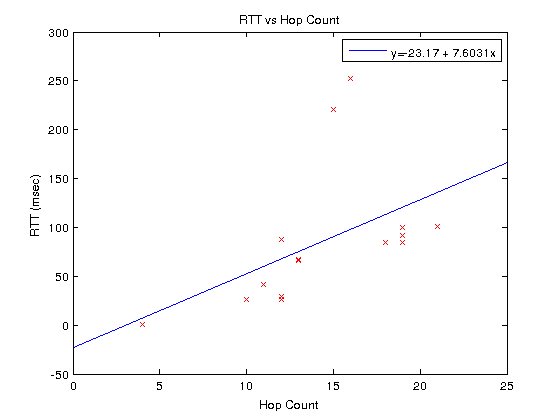
\includegraphics{rtt_vs_hop_count1_legend.png}
  \caption{RTT vs Hop Count}
  \label{fig:scatter1}
\end{figure}
\FloatBarrier

The first scatter plot shown in figure~\ref{fig:scatter1} shows the correlation between RTT and Hop Count. The linear regression for the scatter plot is $y = -23.17 + 7.6031*x$ with an $R^2$ value of $0.245$. This correlation coefficient is not very high (0 is uncorrelated and 1 is perfectly correlated). However, I noticed that there were two main outliers. Looking at the data the outliers were reddit.com and weibo.com. weibo.com was the only site not located in North America so in order to see if within North America there was a stronger correlation I removed weibo.com from the data. Additionally reddit.com was displaying a message about high load at the time that I took measurements. So I removed it from the data set as well.

After removing these two outliers I produced another scatter plot.

\FloatBarrier
\begin{figure}[h!]
  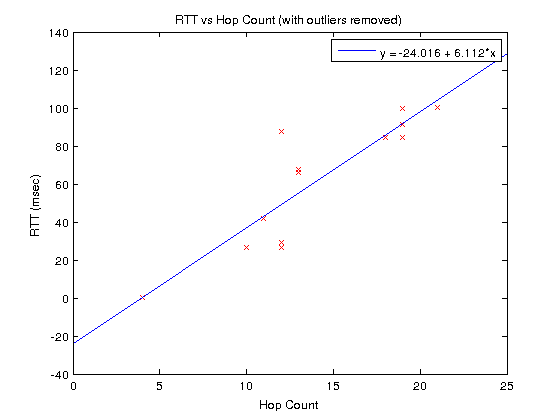
\includegraphics{rtt_vs_hop_count_no_outliers.png}
  \caption{RTT vs Hop Count with reddit.com and weibo.com removed}
  \label{fig:scatter2}
\end{figure}
\FloatBarrier

The new linear regression is $y = -24.016 + 6.112*x$ with an $R^2$ value of $0.783$. This correlation coefficient is much higher and suggests that in general within the continent of North America there is a correlation between RTT and Hop Count. It also suggests that the data is strongly affected by the load of the webservers that are in the data set. Unfortunately it is essentially impossible to measure the load of the servers tested without having administrative access to the servers.

Next I created a scatter plot of distance vs hop count.

\FloatBarrier
\begin{figure}[h!]
  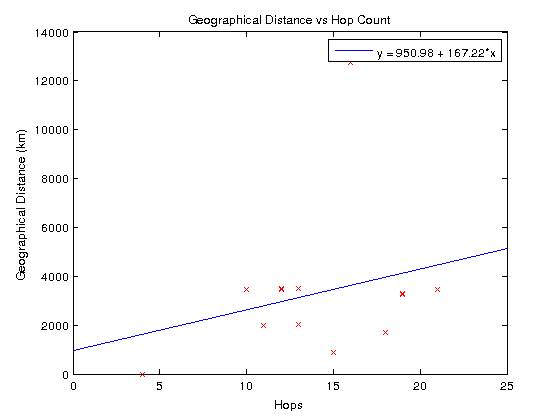
\includegraphics{distance_vs_hop_count1_legend.png}
  \caption{Distance vs Hop Count}
  \label{fig:scatter3}
\end{figure}
\FloatBarrier

The linear regression for this plot is $y = 950.98 + 167.22*x$ with an $R^2$ of $0.0707$. The correlation coefficient is extremely close to 0 showing that for the entire data set distance and hop count are essentially uncorrelated.

Looking at the data with the same two outliers as before removed the scatter plot becomes what is seen if figure~\ref{fig:scatter4}

\FloatBarrier
\begin{figure}[h!]
  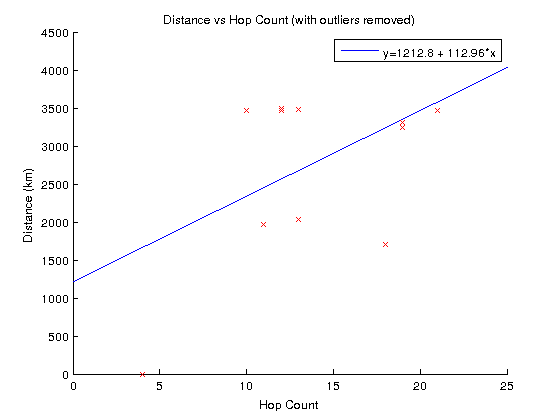
\includegraphics{distance_vs_hop_count_no_outliers.png}
  \caption{Distance vs Hop Count with reddit.com and weibo.com removed}
  \label{fig:scatter4}
\end{figure}
\FloatBarrier

The linear regression for this new plot is $y = 1212.8 + 112.96*x$ with an $R^2$ of $0.258$. This correlation coefficient is higher, but still fairly low indicating that even within the continent hop count is not a good indicator of physical distance.

Finally a scatter plot of distance vs RTT was produced to see if there is a correlation between distance and RTT. The plot is shown in figure~\ref{fig:scatter5}

\FloatBarrier
\begin{figure}[h!]
  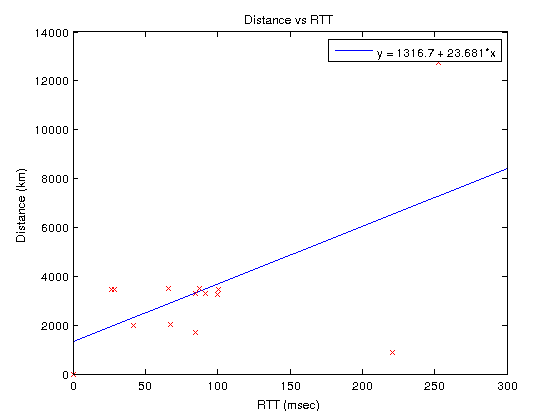
\includegraphics{distance_vs_rtt1_legend.png}
  \caption{Distance vs RTT}
  \label{fig:scatter5}
\end{figure}
\FloatBarrier

The linear regression for this plot is $y = 1316.7 + 23.681*x$ with an $R^2$ of $0.334$. This correlation coefficient is fairly low indicating that RTT is not a good indicator for physical distance. Part of the reason for this may be the inaccuracy in mapping IP addresses to physical locations. The numbers provided by freegeoip.com are simply estimates.

Finally, a scatter plot of distance vs RTT with weibo.com and reddit.com removed was produced. The plot is shown in figure~\ref{fig:scatter6}

\FloatBarrier
\begin{figure}[h!]
  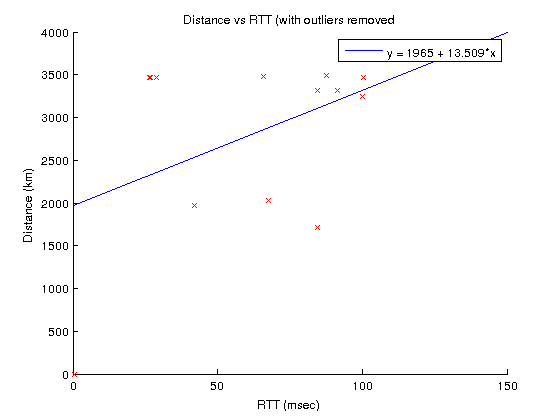
\includegraphics{distance_vs_rtt_no_outliers.png}
  \caption{Distance vs RTT with reddit.com and weibo.com removed}
  \label{fig:scatter6}
\end{figure}
\FloatBarrier

The linear regression for this plot is $y = 1965 + 13.509*x$ with an $R^2$ of $0.176$. This correlation coefficient is even lower. It suggests that there is more variability in RTT for servers on the same continent. Part of this could be due to the error in freegeoip.com's results as if the error is large enough choosing servers closer together will increase the error in my measurements.

\section*{Conclusion}

Overall I find that within the continent hop count is an okay estimator of RTT. Hop Count and RTT have the strongest correlation among each other out of all of the plots produced when only servers within North America are included.

I found that the correlation between distance and RTT actually decreased when only servers within North America were considered suggesting that there is a higher variability in the correlation when servers are located on the same continent.

Finally I found that many sites do not respond to UDP traceroutes, either by silently dropping the packets or by explicitly stating that they have been blocked. This makes it difficult to collect an unbiased sample of data. In order to get around these limitations it would be useful to perform the same test but using ICMP packets and TCP SYN packets to port 80. Many more sites responded to ping's than the UDP traceroute suggesting that an ICMP traceroute could get better data. Additionally because only webservers were tested it is known that all of the servers in the test set should respond to TCP SYN requests on port 80. However, if collecting data this way caution would be needed as the probing could look like a SYN flood attack.

\section*{References}

Traceroute man pages

\end{document}